\documentclass{article}

\usepackage{arxiv}

\usepackage[utf8]{inputenc} % allow utf-8 input
\usepackage[T1]{fontenc}    % use 8-bit T1 fonts
\usepackage{hyperref}       % hyperlinks
\usepackage{url}            % simple URL typesetting
\usepackage{booktabs}       % professional-quality tables
\usepackage{amsfonts}       % blackboard math symbols
\usepackage{nicefrac}       % compact symbols for 1/2, etc.
\usepackage{microtype}      % microtypography
\usepackage{lipsum}		% Can be removed after putting your text content
\usepackage{amssymb,amsmath,amsthm}
\usepackage{listings}
\usepackage{graphicx}
\usepackage{subfig}
\usepackage{apacite}
\usepackage{algorithm}
\usepackage{algorithmicx}
\usepackage{algpseudocode}
\usepackage{kbordermatrix}% http://www.hss.caltech.edu/~kcb/TeX/kbordermatrix.sty
\usepackage{todonotes}

\newtheorem{theorem}{Theorem}
\DeclareMathOperator\supp{supp}

\title{Sampling from the Bayesian poster of an agent-based model given partial observations}

%\date{September 9, 1985}	% Here you can change the date presented in the paper title
%\date{} 					% Or removing it

\author{
  Daniel Tang\\
    Leeds Institute for Data Analytics, University of Leeds, UK\thanks{This project has received funding from the European Research Council (ERC) under the European Union’s Horizon 2020 research and innovation programme (grant agreement No. 757455)}\\
  \texttt{D.Tang@leeds.ac.uk}\\
  \AND
  Nick Malleson\\
  School of Geography, University of Leeds, UK\\  
  %% examples of more authors
  %% \AND
  %% Coauthor \\
  %% Affiliation \\
  %% Address \\
}


\begin{document}
\maketitle

\begin{abstract}
The discipline of data assimilation (DA), sometimes known as data fusion, addresses the problem of how to make use of noisy, imcomplete experimental observations to provide information about the time evolution of unobserved properties of a dynamical system. DA has developed rapidly in applications such as weather forecasting but relatively little progress has been made in developing techniques that are applicable when the dynamical system is an agent based model. ABMs consist of `agents' which often make discrete choices from a number of possible actions, meaning the space of model trajectories is not continuous and we cannot use techniques based on gradient ascent, such as 4D-VAR, that require the gradient of the posterior in this space. In addition, a set of observations will typically refute the vast majority of model trajectories, making it difficult to even identify trajectories that could have given rise to the observations, and so making it challenging to use algorithms that rely on perturbing the current solution such as non-gradient optimisation or most sampling algorithms.

Here we present an algorithm that generates samples of the time evolution of an agent based model, given a set of noisy, incomplete experimental observations of the system. The algorithm approximates the set of possible trajectories as a linear program and uses an extension of the simplex algorithm to provide a proposal function for Markov-Chain-Monte-Carlo sampling.

We demonstrate the algorithm by performing data assimilation in an agent-based, spatial predator-prey model.
\end{abstract}

% keywords can be removed
\keywords{Data assimilation, Bayesian inference, Agent based model, Integer linear programming, predator prey model}

\section{Introduction}

\todo[inline]{NM: Paragraph for intro / context}

Data assimilation (DA) is a technique that has been widely used in the physical sciences such as meteorology~\cite{kalnay_atmospheric_2003}, oceanography~\cite{bertino_sequential_2003} and the earth sciences more broadly~\cite{reichle_data_2008}. Specific applications of DA to ABMs are, however, much rarer. Examples of data assimilation using well-known DA methods such as Particle Filters and variants of the Kalman Filter applied to ABMs include models of crime~\cite{lloyd_exploring_2016}, bus routes~\cite{kieu_dealing_2020}, pedestrian dynamics~\cite{wang_data_2015, ward_dynamic_2016, clay_realtime_2020, malleson_simulating_2020};
and population movement~\cite{lueck_who_2019}. Many DA algorithms rely on the differentiability of the model~\cite{lewis_dynamic_2006}.
\todo[inline]{NM: More detail on drawbacks and limitations of those approaches}

\todo[inline]{NM: Aims of this paper and knowledge gap it fills.}

\todo[inline]{NM: ``This paper has been structured as follows ... ''}

\section{Formulation of the problem}
%##########################################

Suppose we have a timestepping ABM where agents have a finite number of possible internal states and a finite number of ways of acting on their world. Given this, we can define an ABM as:
\begin{itemize}
	\item A vector of agent actions $\mathcal{A} =\left< A_0 ... A_n \right>$
	
	\item A vector of agent states $\mathcal{S} = \left<S_0 ... S_m\right>$
	
	\item An \textit{agent timestep}, $\pi : \mathbb{Z}\times\mathbb{Z}^{m+1}\times\mathbb{Z} \to \mathbb{R}$, which defines the probability that an agent will act in a particular way such that $\pi(\psi,\Phi,a)$ gives the probability that an agent in state $S_\psi$, surrounded by agents, $\Phi$, will perform action $A_a$ (where $\Phi$ is a vector whose $i^{th}$ element is the number of agents in state $S_i$ at the start of the timestep).
	
	\item An \textit{action function}, $F: \mathbb{Z} \times \mathbb{Z} \to \mathbb{Z}^{m+1}$, which defines the effect of an action on the world such that $F(\psi, a)$ returns a vector, $\Phi$, whose $i^{th}$ element gives the number of agents in state $S_i$ that result from an agent in state $S_\psi$ performing act $A_a$ (including the final state of the acting agent).
\end{itemize}

As a simple illustration, consider the simple ``cat and mouse'' ABM, which consists of just two gridsquares, left and right, within which can roam cats and mice, so the vector of agent states is, $\mathcal{S} = \left<\textrm{left cat}, \textrm{right cat}, \textrm{left mouse}, \textrm{right mouse} \right>$. In any given timestep, agents can either move or stay still, so the vector of actions is $\mathcal{A} = \left<\textrm{move}, \textrm{stay still}\right>$.

A cat moves with probability $0.5$, irrespective of other agents, while a mouse will move if there is one or more cats on the same gridsquare, otherwise it will stay still. So, the agent timestep function is
\begin{equation}
\begin{aligned}
\pi(\psi, \Phi, 0) &=
\begin{cases}
0.5 & \text{if } \psi \in \left\{0,1\right\}\\
1 & \text{ if } \psi = 2, \Phi_1 > 0 \text{ or } \psi=3, \Phi_2 > 0\\
0 & \text{ otherwise}
\end{cases}\\
\pi(\psi, \Phi, 1) &=
\begin{cases}
0.5 & \text{if } \psi \in \left\{0, 1\right\}\\
1 & \text{ if } \psi = 2, \Phi_1 = 0 \text{ or } \psi=3, \Phi_2 = 0\\
0 & \text{ otherwise}
\end{cases}
\end{aligned}
\end{equation}

The action function expresses the movement of the agents
\begin{equation}
\begin{aligned}
F(0, 0) &= \{0,1,0,0\}\\
F(1, 0) &= \{1,0,0,0\}\\
F(2, 0) &= \{0,0,0,1\}\\
F(3, 0) &= \{0,0,1,0\}\\
F(0, 1) &= \{1,0,0,0\}\\
F(1, 1) &= \{0,1,0,0\}\\
F(2, 1) &= \{0,0,1,0\}\\
F(3, 1) &= \{0,0,0,1\}\\
\end{aligned}
\end{equation}

\subsection{Trajectories}

\begin{figure}
	\centering
	\resizebox{0.5\textwidth}{!}{
		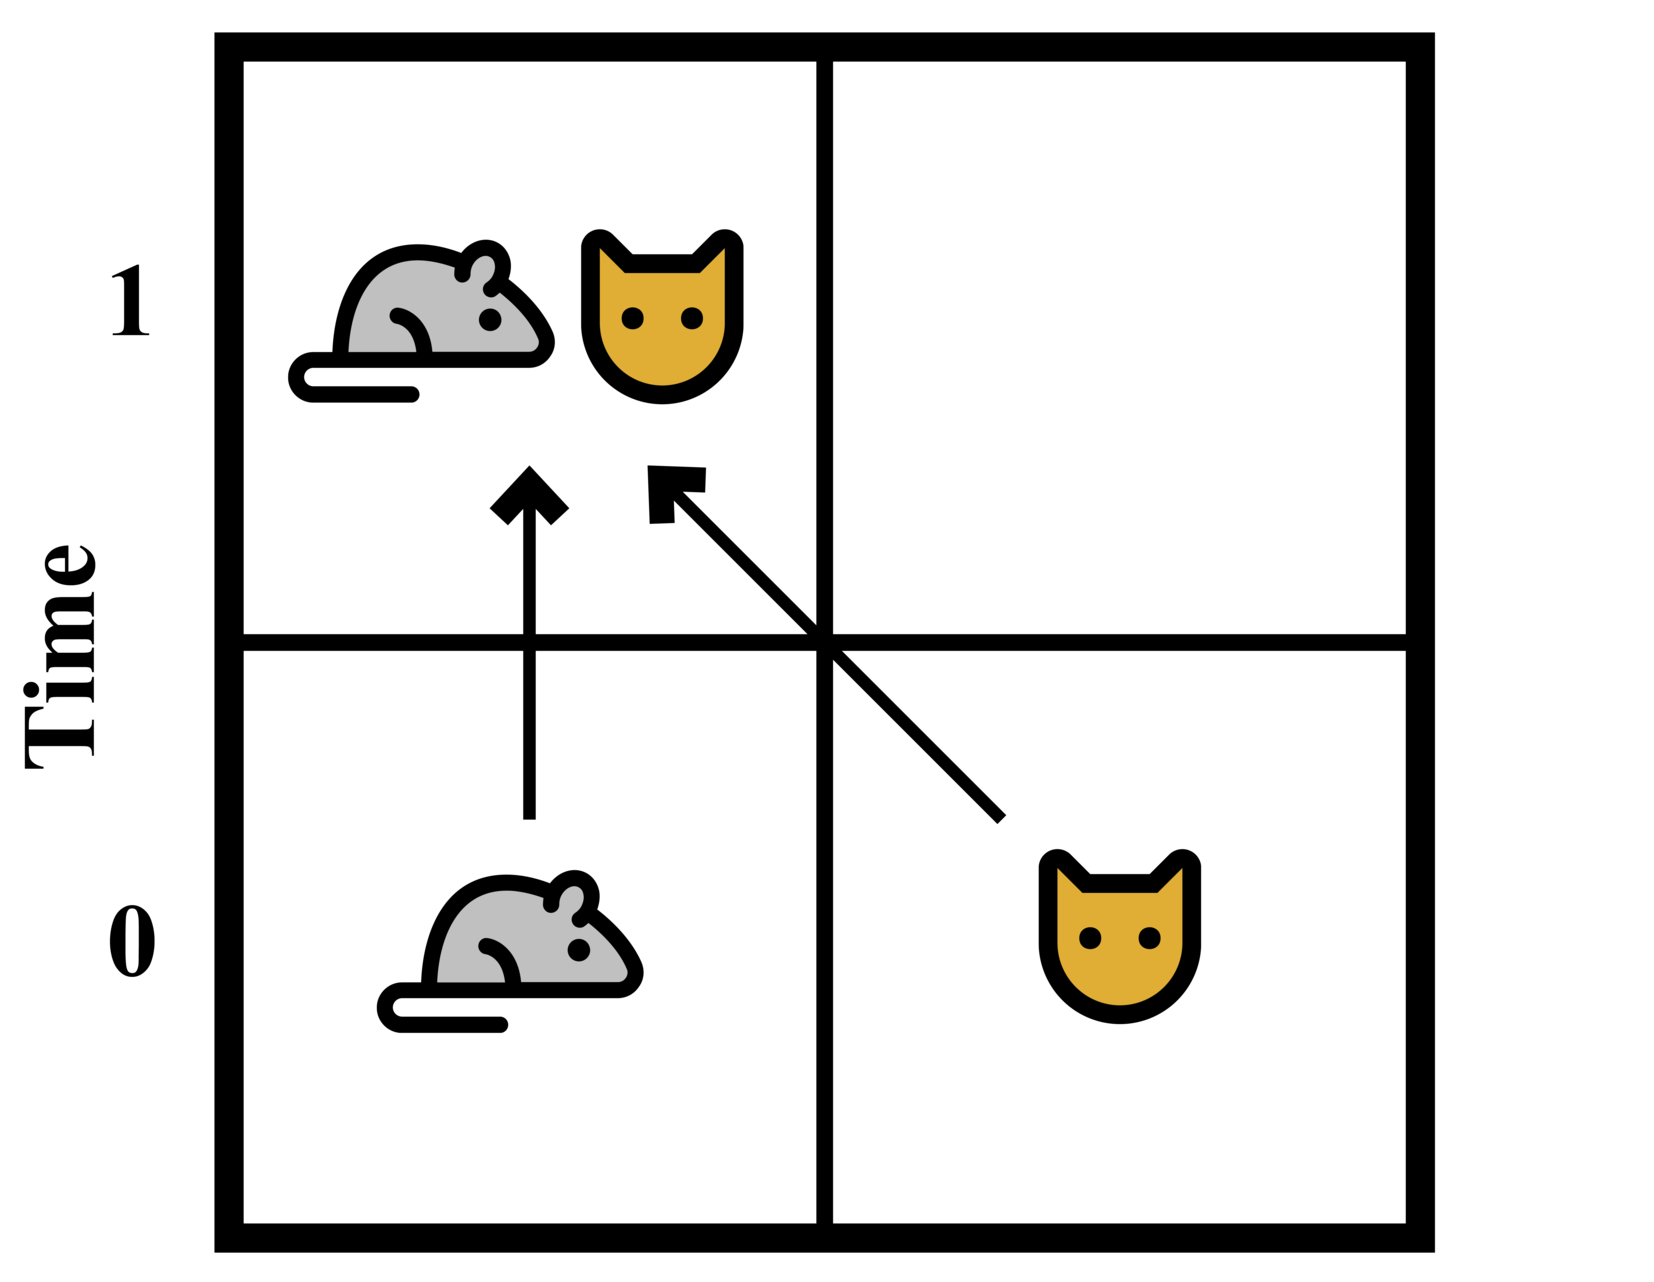
\includegraphics[scale=0.5]{figs/catMouseSm}
	}
	\caption{A simple cat and mouse model.\label{fig:AB-MCMC-1}}
\end{figure}


Let a model timestep consist of a matrix $E$ whose elements $e_{\psi a}$ are the number of agents in state $\psi$ that perform act $a$ in this timestep. For example, the timestep shown in Figure~\ref{fig:AB-MCMC-1} for the cat and mouse example would be
\[
E = \kbordermatrix{
	& A_0 & A_1 \\
	S_0 & 0 & 0 \\
	S_1 & 1 & 0 \\
	S_2 & 0  & 1 \\
	S_3 & 0 & 0 \\
}
\]
where all elements are zero except those representing agent $S_1$ performing action $A_0$ and agent $S_2$ performing action $A_1$.

Finally, let a model trajectory be a tensor, $T$, consisting of a number of model timesteps. We use the notation $T^t$ to denote the $t^{th}$ timestep matrix, $T^t_\psi$ to denote the $\psi^{th}$ row of the $t^{th}$ timestep matrix and $T^t_{\psi a}$ to denote the $a^{th}$ element of the $\psi^{th}$ row of the $t^{th}$ timestep. By convention, we'll let indices begin at 0. Note that this tensor will generally be very large for more realistic models, but also very sparse, so it can be dealt with computationally using a sparse representation.

It will occasionally be useful to refer to the set of all tensors of a given shape. For this we'll use $\mathbb{R}$ adorned with the number of elements in each index position. For example, a trajectory representing $N$ timesteps of a model with $S$ agent states and $A$ actions must be a member of the set of tensors $\mathbb{R}^N_{SA}$.

A tensor must satisfy a number of constraints in order to be a valid trajectory of an ABM. Since the elements of a trajectory are counts, they must all be non-negative integers, we'll call this the \textit{non-negative integer constraint} and define the set of all non-negative integer tensors
\begin{equation}
\mathcal{I}^N_{SA} = \left\{ T \in \mathbb{R^N_{SA}}: \forall t,\psi, a: T^t_{\psi a} \ge 0, T^t_{\psi a} \in \mathbb{Z}\right\}
\label{nonNegativeInt}
\end{equation}

A trajectory must also be \textit{continuous} by which we mean that the number of agents in each state at the end of timestep $t-1$ must be the number of agents in each state at the beginning of timestep $t$. We call this the \textit{continuity constraint} and define the set of continuous tensors:
\begin{equation}
\mathcal{C}^N_{SA}(F) = \left\{T\in\mathbb{R}^N_{SA}:  \forall t \in 1 ... N-1:\forall \phi: \sum_{\psi, a} F(\psi, a)_\phi T^{t-1}_{\psi a} - \sum_a T^t_{\phi a} = 0\right\}
\label{continuous}
\end{equation}

So, the set of valid trajectories, $\mathcal{T}^N_{SA}(F)$, is given by the set of tensors that satisfy \ref{nonNegativeInt} and \ref{continuous}.
\begin{equation}
\mathcal{T}^N_{SA}(F) = \mathcal{I}^N_{SA} \cap \mathcal{C}^N_{SA}(F)
\end{equation}


\subsection{The posterior}

If we let $\Psi^t$ be the vector whose $\psi^{th}$ element is the number of agents in state $S_\psi$ at the beginning of timestep $t$, then the prior probability of a trajectory is
\[
P(T) =
\begin{cases}
P\left(\Psi^0 = T^0 \mathbf{1} \right) \prod_{\psi, t} P\left(T^t_{\psi} \mid \Psi^t = T^t \mathbf{1}\right) & \text{if } T \in \mathcal{T}^N_{SA}(F) \\
0 & \text{otherwise}
\end{cases}
\]
where $P(\Psi^0)$ is our prior beliefs about the state at time $t=0$, and we use $\mathbf{1}$ to denote a vector whose elements are all 1.


The probability that a single agent in a given state will perform an action, given the state of the other agents, $\Psi^t$, is given by the agent timestep function, $\pi(\psi,\Psi^t,a)$, so the joint probability that $\Psi^t_\psi$ agents will perform actions $T^t_{\psi}$ in an environment of other agents $\Psi^t$, is given by the multinomial distribution
\[
P\left(T^t_{\psi} \mid \Psi^t \right) = \Psi^t_\psi!\prod_a \frac{\pi(\psi,\Psi^t,a)^{T^{t}_{\psi a}}}{T^{t}_{\psi a}!}.
\]
So the prior probability of a trajectory is
\[
P(T) =
\begin{cases}
P(\Psi^0 = T^0\mathbf{1})
\prod_{t, \psi}\left(T^t_{\psi} \cdot \mathbf{1} \right)!
\prod_a \frac{\pi(\psi, T^{t}\mathbf{1},a)^{T^{t}_{\psi a}}}{T^{t}_{\psi a}!} & \text{if } T \in \mathcal{T}^N_{SA}(F) \\
0 & \text{otherwise}\\
\end{cases}
\]

Suppose now we have a set of noisy, aggregate observations, $\Omega$, that have a likelihood function $P(\Omega|T)$. By Bayes' rule, we have
\[
P(T|\Omega) \propto P\left(\Omega \middle| T\right)P(T)
\]

Without loss of generality, we take $\Omega$ to consist of some number of observations that are independent of each other given the trajectory, so that the members $(\omega,v)\in \Omega$ consist of a stochastic observation operator $\omega$ and an observed value $v$ (which may be a vector). We write $P(\omega(T)=v)$ to denote the probability of observation operator $\omega$ making observation $v$ on trajectory $T$. So
\[
P(\Omega|T) = \prod_{(\omega,v) \in \Omega} P(\omega(T)=v)
\]

The posterior can now be written as
\begin{equation}
P(T|\Omega) \propto 
\begin{cases}
P(\Psi^0 = T^0\mathbf{1})
\prod_{(\omega,v) \in \Omega} P\left(\omega(T)=v\right)
\prod_{t, \psi, a}\left(T^t_{\psi}\cdot\mathbf{1}\right)!
\frac{\pi(\psi,T^t\mathbf{1},a)^{T^{t}_{\psi a}}}{T^t_{\psi a}!} & \text{if } T \in \mathcal{T}^N_{SA}(F) \\
0 & \text{otherwise}\\
\end{cases}
\label{posterior}
\end{equation}

The problem we're interested in is how to sample from this distribution. In many practical applications, sampling is difficult because the posterior has zero probability for the vast majority of tensors (i.e. most tensors are not trajectories, contain an impossible action or are refuted by the observations). Even though we can generate trajectories that fit the prior by simply performing a forward execution of the model from an initial state drawn from the prior, if the observations refute the trajectory the probability falls to zero. It doesn't take many observations until the probability of randomly choosing a trajectory that fits the observations becomes very small indeed. So simple techniques such as rejection sampling, for example, are not practical. Techniques based on particle filtering may have more success but, for similar reasons, will likely soon reach a state containing a set of particles, none of which can be fit to the observations.

In this paper we'll show how the Metropolis-Hastings algorithm can be used to generate samples from equation \ref{posterior}. The challenge will be to create a proposal function which randomly generates a proposed next sample given the current one. For example, a common strategy with Metropolis-Hastings is to generate a new sample by perturbing one or more elements of the previous sample at random. However, if we do this with an ABM trajectory it's very unlikely that the perturbed tensor will be a trajectory that contains only possible actions and satisfies the observations. So, the proposed next sample would almost certainly be rejected and we'd probably end up stuck on the first sample until we grew old.

\section{Approximating the support of the posterior}
%##########################################

We solve this problem by first approximating the support of the posterior, $\supp(P(T^t_{\psi a}|\Omega))$ (i.e. the set of trajectories that have non-zero probability).

From equation \ref{posterior}
\begin{equation}
\begin{aligned}
\supp (P( T |\Omega)) = & \mathcal{T}^N_{SA} \cap \\ 
&\supp(P(\Psi^0 = T^0\mathbf{1})) \cap \\
&\bigcap_{(\omega,v) \in \Omega}  \supp\left(P\left(\omega(T)=v\right)\right) \cap \\
&\bigcap_{t, \psi, a} \left( \supp\left(\pi(\psi,T^t\mathbf{1},a)\right) \cup \left\{T:T^t_{\psi a} = 0\right\} \right)
\end{aligned}
\label{support}
\end{equation}
i.e. in order for $T$ to have non-zero posterior probability, it must be a trajectory of the ABM, it must have a start state that has non-zero prior probability, all the observation likelihoods must be non-zero and each element of $T$ must either denote an agent action with non-zero probability or must be equal to zero (to account for the fact that $0^0=1$ in the exponent terms in \ref{posterior}).

\subsection{Fermionic Trajectories}

In the following we will consider only \textit{Fermionic trajectories}, which we define to be any trajectory whose elements are all either 0 or 1. i.e. a Fermionic trajectory must not only satisfy the constraints in \ref{nonNegativeInt} and \ref{continuous} but must also satisfy the \textit{Fermionic constraints}
\begin{equation}
\mathcal{B}^N_{SA} = \left\{T\in\mathbb{R}^N_{SA} : \forall t,\psi,a: T^t_{\psi a} \in \left\{ 0,1 \right\}\right\}
\label{fermionic}
\end{equation}
This can be interpreted as meaning that no two agents in the same state at the same time can perform the same action. Notice that the Fermionic constraints imply the non-negative integer constraints, so the set of Fermionic trajectories, $\mathcal{F}^N_{SA}$, is the set of tensors that satisfy \ref{fermionic} and \ref{continuous}.
\begin{equation}
\mathcal{F}^N_{SA}(F) = \mathcal{B}^N_{SA} \cap \mathcal{C}^N_{SA}(F)
\end{equation}

If we now condition the posterior on $T \in \mathcal{B}^N_{SA}$ then the support of the posterior becomes
\begin{equation}
supp(P(T|\Omega, T\in\mathcal{B}^N_{SA})) = \mathcal{B}^N_{SA} \cap supp(P(T|\Omega))
\label{fermionicSupport1}
\end{equation}

In practice, the number of agents in an ABM is usually much smaller than the number of agent states, so it is overwhelmingly likely that a sample from the posterior will be Fermionic, and so intersection with $\mathcal{B}^N_{SA}$ will often have very little effect on the posterior. However, section ** describes how to extend the algorithm to apply to non-Fermionic trajectories when the Fermionic constraints are not acceptable.

\subsection{Convex $\mathcal{B}$-polyhedra and $\mathcal{B}$-distributions}
%################################################################
\label{BPoly}

We define a $\mathcal{B}$-polyhedron to be a set of binary vectors
\[
\mathcal{B}^N_{SA} \cap \mathcal{P}
\]
where $\mathcal{P} \subset \mathcal{R}^N_{SA}$ is a convex polyhedron in the sense that it can be expressed as a set of tensors that satisfy some number of linear constraints on their elements. More formally, there exists a tensor $C \in \mathbb{R}^{SA}_{NJ}$ and vectors $L \in \mathbb{R}_J$ and $U \in \mathbb{R}_J$ such that:
\[
\mathcal{P} = \left\{ T\in\mathbb{R}^N_{SA} : L \le \sum_{t,\psi,a} C^{\psi a}_{t} T^t_{\psi a} \le U \right\}
\]

\begin{theorem}
For any set $\mathcal{X}$ there exists a convex polyhedron $P$ such that
\[
\mathcal{B}^N_{SA} \cap \mathcal{X} = \mathcal{B}^N_{SA} \cap \mathcal{P}
\]
\end{theorem}
\begin{proof}
Let $\mathcal{Y} = \mathcal{B}^N_{SA} \cap \mathcal{X}$ and let $\mathcal{P}$ be the convex hull of $\mathcal{Y}$. Clearly if a tensor $T\in \mathcal{Y}$ then $T\in \mathcal{B}^N_{SA} \cap \mathcal{P}$. To show the converse, suppose there is a member $T' \in \mathcal{B}^N_{SA} \cap \mathcal{P}$. Since $T'\in \mathcal{P}$ then there must be a convex combination of points in $\mathcal{Y}$ that equals $T'$. Call those points $\mathcal{Z}$. However, since $T' \in \mathcal{B}^N_{SA}$ and $\mathcal{Z}\subset \mathcal{B}^N_{SA}$ and no member of $\mathcal{B}^N_{SA}$ is a convex combination of any other member then $T'$ must be a member of $\mathcal{Z}$ and so $T'\in \mathcal{Y}$. So $\mathcal{B}^N_{SA} \cap \mathcal{X} = \mathcal{B}^N_{SA} \cap \mathcal{P}$. 
\end{proof}

Under the assumption that all trajectories are Fermionic, we can rewrite equation \ref{support} in the form
\begin{equation}
\begin{aligned}
\mathcal{B}^N_{SA} \cap \supp (P( T |\Omega)) = 
& \mathcal{B}^N_{SA} \cap \mathcal{C}^N_{SA}(F) \cap \\
& \mathcal{B}^N_{SA} \cap  \supp(P(\Psi^0 = T^0\mathbf{1})) \cap\\
& \bigcap_{(\omega,v) \in \Omega}   \mathcal{B}^N_{SA} \cap \supp\left(P\left(\omega(T)=v\right)\right) \cap \\
& \bigcap_{t,\psi, a}
\mathcal{B}^N_{SA} \cap \left(\supp\left(\pi(\psi,T^t\mathbf{1},a)\right)
\cup
\left\{T: T^t_{\psi a} = 0\right\}\right)
\\
\end{aligned}
\label{fermionicSupport}
\end{equation}
which is an intersection of terms in the form $\mathcal{B}^N_{SA} \cap \mathcal{X}$, so each term can equivalently be expressed as a $\mathcal{B}$-polyhedron.

The union in the last line would be inconvenient to deal with computationally so we transform it away in the following way. Let $\mathcal{P}^t_{\psi a}$ be a convex polyhedron such that
\[
\mathcal{B}^N_{SA} \cap \mathcal{P}^t_{\psi a} = \mathcal{B}^N_{SA} \cap \supp\left(\pi(\psi,T^t\mathbf{1},a)\right)
\]
so
\[
\mathcal{B}^N_{SA} \cap \left(\supp\left(\pi(\psi,T^t\mathbf{1},a)\right) \cup
\left\{T: T^t_{\psi a} = 0\right\}\right)
=
\mathcal{B}^N_{SA} \cap \left(\mathcal{P}^t_{\psi a} \cup \left\{T: T^t_{\psi a} = 0\right\}\right)
\]
If we let
\[
\mathcal{P}^t_{\psi a} = \left\{ T\in\mathbb{R}^N_{SA} : L \le \sum_{s,\phi,b} C^{\phi b}_{s} T^s_{\phi b} \le U \right\}
\]
for some $C \in \mathbb{R}^{SA}_{NI}$ and $L\in\mathbb{R}_I$ and $U\in\mathbb{R}_I$ then we can remove the union using the identity
\begin{multline}
\mathcal{B}^N_{SA} \cap
\left(
\left\{ T\in\mathbb{R}^N_{SA} : L \le \sum_{s,\phi,b} C^{\phi b}_{s} T^s_{\phi b} \le U \right\}
\cup
\left\{T: T^t_{\psi a} = 0\right\}\right)
=\\
\mathcal{B}^N_{SA} \cap
\left\{
T\in\mathbb{R}^N_{SA}:
-\infty \le \sum_{s,\phi,b} C^{\phi b}_{s} T^s_{\phi b}
+
(\overline{B}-U)T^{t}_{\psi a}
\le \overline{B}
\right\}
\cap\\
\mathcal{B}^N_{SA} \cap
\left\{
T\in\mathbb{R}^N_{SA}:
\underline{B} \le \sum_{s,\phi,b} C^{\phi b}_{s} T^s_{\phi b}
+
(\underline{B}-L)T^{t}_{\psi a} \le \infty
\right\}
\label{implication}
\end{multline}
where the elements of $\overline{B}\in\mathbb{R}_I$ are defined as
\[
\overline{B}_i = \frac{\sum_{s,\phi,b} \left( |C^{\phi b}_{si}| + C^{\phi b}_{si}\right)}{2}
\]
and the elements of $\underline{B}\in\mathbb{R}_I$ are defined as
\[
\underline{B}_i = \frac{\sum_{s,\phi,b} \left( |C^{\phi b}_{si}| - C^{\phi b}_{si}\right)}{2}
\]

To see why this identity holds, consider the right hand polyhedrons in \ref{implication}. When $T^t_{\psi a}=1$ the first is equal to $\sum_{s,\phi,b} C^{\phi b}_{s} T^s_{\phi b} \le U$ and the second is equal to $L \le \sum_{s,\phi,b} C^{\phi b}_{s} T^s_{\phi b}$ so their intersection is $\mathcal{P}^t_{\psi a}$, whereas when $T^t_{\psi a}=0$ the right hand side terms give $\underline{B} \le \sum_{s,\phi,b} C^{\phi b}_{s} T^s_{\phi b} \le \overline{B}$. But the elements $\underline{B}_i$ and $\overline{B}_i$ are an lower and upper bounds on the value of $\sum_{s,\phi,b} C^{\phi b}_{si} T^s_{\phi b}$ given that $T\in\mathcal{B}^N_{SA}$, so this is satisfied for all $\mathcal{B}^N_{SA}$ such that $T^t_{\psi a}=0$.

Using this transformation the Fermionic support of the posterior can be reduced to the intersection of $\mathcal{B}$-polyhedra. Given the identity
\[
(\mathcal{B}^N_{SA} \cap P_1) \cap (\mathcal{B}^N_{SA} \cap P_2) = \mathcal{B}^N_{SA} \cap (P_1 \cap P_2)
\]
we can calculate \ref{fermionicSupport}, and thereby represent the support of the posterior as a set of linear constraints, by calculating each term and simply concatenating their linear constraints.

The idea of a $\mathcal{B}$-polyhedron as the support for a probability distribution naturally leads to the idea of a $\mathcal{B}-distribution$ which is a probability distribution which is a discrete distribution defined on the points of a $\mathcal{B}-polyhedron$. From the above, it can be seen that the posterior distribution of an ABM trajectory is a $\mathcal{B}-distribution$.

As an illustration, consider two timesteps of the cat and mouse model. Suppose we flip a fair coin to decide whether each agent state is occupied or empty at $t=0$ and that we observe a cat in the left grid-square at time $t=1$. Our aim is to construct a set of linear constraints, $Q$, such that
\[
\mathcal{B}^2_{4\,2} \cap \supp(P(T|\Omega)) = \mathcal{B}^2_{4\,2} \cap Q
\]
Working through \ref{fermionicSupport} term by term, the $\mathcal{B}^N_{SA} \cap \mathcal{C}^N_{SA}(F)$ term is equivalent to a $\mathcal{B}$-polyhedron with the continuity constraints in \ref{continuous}, which are already in linear form so we're done. The second term is the support of the prior. This constrains each agent state at $t=0$ to be at most 1, which can be expressed as
\[
\bigcap_\psi \left\{T:T^0_{\psi 0} + T^0_{\psi 1} \le 1\right\}
\]

The third term is the support of the observation. Since we observe a cat in the left grid-square at time $t=1$ we need to add the constraint
\[
T^1_{0 0} + T^1_{0 1} = 1
\]
The final term guards against impossible actions. The only impossible actions are a mouse staying put when there is a cat on the same gridsquare or moving when there are no cats, which translates to the four cases
\[
\begin{aligned}
\supp(\pi(2,T^t\mathbf{1},0)) &= \left\{ T: -T^t_{0 0} - T^t_{0 1} \le -1 \right\}\\
\supp(\pi(3,T^t\mathbf{1},0)) &= \left\{ T: -T^t_{1 0} - T^t_{1 1} \le -1 \right\}\\
\supp(\pi(2,T^t\mathbf{1},1)) &= \left\{ T: T^t_{0 0} + T^t_{0 1} \le 0 \right\}\\
\supp(\pi(3,T^t\mathbf{1},1)) &= \left\{ T: T^t_{1 0} + T^t_{1 1} \le 0 \right\}
\end{aligned}
\]
Using the identity in \ref{implication} to take the union of each of these with $\left\{T: T^t_{\psi a} = 0\right\}$ gives the four constraints
\[
\begin{aligned}
-T^t_{0 0} - T^t_{0 1} + T^t_{2 0} & \le 0\\
-T^t_{1 0} - T^t_{1 1} + T^t_{3 0} & \le 0\\
T^t_{0 0} + T^t_{0 1} + 2T^t_{2 1} & \le 2 \\
T^t_{1 0} + T^t_{1 1} + 2T^t_{3 1} & \le 2
\end{aligned}
\]
for each timestep $t=0$ and $t=1$.

Taken together, these constraints define a $\mathcal{B}$-polyhedron that is the set of Fermionic trajectories for the cat and mouse ABM, and when combined with equation \ref{posterior} defines $P(T|\Omega)$ as a $\mathcal{B}-distribution$.

\section{Transforming between representations of a $\mathcal{B}$-polyhedron}
%#####################################################

Now that we can express the support of the posterior as a $\mathcal{B}$-polyhedron in the form
\begin{equation}
\supp(P(T|\Omega) = \mathcal{B}^N_{SA} \cap \left\{T: L \le \sum_{t,\psi,a} C^{\psi a}_t T^t_{\psi a} \le U \right\}
\label{bPolySupport}
\end{equation}
we now describe some different ways of representing the same $\mathcal{B}$-polyhedron and methods of transforming from one representation to another. This will be useful in the development that follows.

\subsection{The standard form of a $\mathcal{B}$-polyhedron}

Since there are many ways of representing a polyhedron, it will be useful to define a standard form when representing $\mathcal{B}$-polyhedra. We'll use the form
\begin{equation}
\mathcal{B}(Q,N,b,L,U) = \left\{X: X = Q{X_B\choose X_N}, X_B = NX_N + b, X_B\in\mathbb{Z}^I, L \le X_B \le U, X \in \left\{ 0,1\right\}^K, X_N \in \left\{0,1\right\}^J \right\}
\label{standardpolyhedron}
\end{equation}
where $X\in \mathbb{R}^K$, $X_N\in\mathbb{R}^J$ and $X_B\in\mathbb{R}^I$ are now vectors and $Q$ is a $K\times (I+J)$ matrix that selects $J \le K \le I+J$ elements from $(X_B|X_N)^T$ (i.e. each column of $Q$ has at most one element equal to 1, each row has exactly one element equal to 1 and all other elements are 0). We'll call the elements of $X_B$ ``basic-variables'' and the elements of $X_N$ ``non-basic variables''\footnote{The introduction of the requirement that $X_B \in \mathbb{Z}$ does not reduce expressivity as long as the elements of $N$ and $b$ can be expressed as rational numbers. In this case they can be converted to integers by multiplying each row by the product of the denominators on that row and dividing by the greatest common divisor. Once $N$ and $b$ are integer then $X_B$ is guaranteed to be integer for any $X_N\in\{0,1\}^J$.}.

Equation \ref{bPolySupport} can easily be expressed in the form \ref{standardpolyhedron} by ``flattening'' the trajectory, $T$, into a $J$-dimensional vector (without changing the values of the elements) using a tensor $R\in\mathbb{R}^{SA}_{NJ}$ where $J=NSA$ (i.e. for every $(t, \psi, a)$ there is exactly one $j$ such that $R^{\psi a}_{t j} = 1$ and for every $j$ there is exactly one $(t,\psi,a)$ such that $R^{\psi a}_{t j} = 1$ and all other elements are zero) so that
\[
X_N = \sum_{t,\psi,a}R^{\psi a}_t T^t_{\psi a}
\]
and letting $N$ be the $I\times J$ matrix
\[
N = \sum_{t,\psi,a} C^{\psi a}_t R^{\psi a}_t
\]
and finally letting Q be the matrix such that $X_N = Q(X_B|X_N)$ and $b = \mathbf{0}$. The constraint $X_B\in\mathbb{I}^I$ is satisfied since all the elements of $N$ are integers in our case.

\subsection{The pivot transformation}

The introduction of the matrix $Q$ in \ref{standardpolyhedron} allows us to transform the representation without changing the $\mathcal{B}$-polyhedron that is represented. We now describe the ``pivot transformation'' which will be a central operation in the sampling algorithm, and should look familiar to anyone acquainted with the simplex algorithm (see e.g. \cite{vanderbei2015linear}).

We begin by transforming \ref{standardpolyhedron} to the equivalent form
\begin{equation}
\mathcal{B} = \left\{X: X = Q{X_B\choose X_N}, (I|-N){X_B\choose X_N} = b, {L\choose \mathbf{0}} \le {X_B \choose X_N} \le {U\choose \mathbf{1}}, X \in \left\{ 0,1\right\}^K, {X_B\choose X_N} \in \mathbb{I}^{I+J} \right\}
\label{joinedpolyhedron}
\end{equation}

If we let $S_{ij}$ be the permutation matrix such that
\[
{X'_B\choose X'_N} = S_{ij}{X_B\choose X_N}
\]
has the effect of swapping the $i^{th}$ element of $X_B$ with the $j^{th}$ element of $X_N$ then we can change variables in the equality constraint so that
\[
(I|-N)S^{-1}_{ij}{X'_B \choose X'_N} = b
\]
(note that $S^{-1}_{ij} = S_{ij}$).

However, the matrix $(I|-N)S^{-1}_{ij}$ is no longer in the standard form since $S^{-1}_{ij}$ has the effect of replacing a column in the identity with a column in the $-N$ matrix, leaving the first $I$ columns of $(I|-N)S^{-1}_{ij}$ equal to
\[
B = (I|-N)S^{-1}_{ij}{I \choose \mathbf{0}}
\]
which is not, in general, the identity. However, as long as $N_{ij} \ne 0$ then $B$ is invertible, having the simple form
\[
B^{-1} =  
\begin{pmatrix}
1 &  & -\frac{N_{0j}}{N_{ij}} & & \\
  & \ddots & \vdots & &\\
 & & \frac{1}{-N_{ij}} & &\\
  & & \vdots & \ddots &\\
  & & -\frac{N_{nj}}{N_{ij}} & &1\\
\end{pmatrix}
\]
We can now recover the standard form by pre-multiplying by $B^{-1}$
\[
B^{-1}(I|-N)S^{-1}_{ij} = (B^{-1}|-B^{-1}N)S^{-1}_{ij} = (I|-N') = B^{-1}b  = b'
\]
Since $B^{-1}$ is invertible the transformed constraint is equivalent to the original, so if we let
\[
Q' = QS^{-1}_{ij}
\]
we can express $\mathcal{B}$ in the form
\begin{equation}
\mathcal{B} = \left\{X: X = Q'{X'_B\choose X'_N}, (I|-N'){X'_B\choose X'_N} = b', S_{ij}{L\choose \mathbf{0}} \le {X'_B \choose X'_N} \le S_{ij}{U\choose \mathbf{1}}, X \in \left\{ 0,1\right\}^K, {X'_B\choose X'_N} \in \mathbb{I}^{I+J} \right\}
\end{equation}

This is almost in the standard form, apart from the lower and upper bounds on $X'_N$ which may have an element with bounds other than 0 and 1. However, if we add the constraint that a pivot transformation can only be performed for $i: L_i = 0, U_i=1$ then $S_{ij}$ makes no change and the transformed representation is standard.

It is easy to see that this transformation can be extended to any permutation matrix $S$ such that $B = (I|-N)S^{-1}(I|\mathbf{0})^T$ is invertible. So, given a reference representation of a $\mathcal{B}$-polyhedron, $\mathcal{B}(Q,N,b,L,U)$, we can define the set of all equivalent ``pivot states'' with respect to $(N,L,U)$ to be
\[
\mathcal{S}(N,L,U) = \left\{S : S \text{ is a permutation matrix }, (I|-N)S^{-1}{I\choose \mathbf{0}} \text{ is invertible}, \exists L',U': S{L|U \choose \mathbf{0}|\mathbf{1}} = {L'|U' \choose \mathbf{0}|\mathbf{1}} \right\}
\]
so that each pivot state, when applied to the reference state, gives an equivalent standard form representation.

\subsection{Removal of fixed variables}

If we use the method described in section \ref{BPoly} to create a $\mathcal{B}$-polyhedron of the support then each continuity constraint (and possibly some of the observation constraints) will result in elements of $X_B$ that have fixed values (i.e. $L_i = U_i$). Removing these will reduce the dimensionality of the problem and so make valid solutions easier to find.

Suppose the $i^{th}$ element of $X_B$ is fixed. We can perform a pivot on $(i,j)$, for some $j:N_{ij}\ne 0$ to swap the fixed variable with the $j^{th}$ element of $X_N$ so that the fixed variable ends up in $X_N$. This would leave the upper and lower bounds in a non-standard state since $X_N$ must have bounds $\mathbf{0} \le X_N \le \mathbf{1}$. However, the fixed variable can be removed from $X_N$ by adding the $j^{th}$ column of $N$ times the fixed variable to left and right sides of the equality constraint.
\[
(I|-N){X_B \choose X_N} + N^jX_{Nj} = b + N^jX_{Nj} = (I|-N'){X_B \choose X'_N} = b'
\]
where $N^j$ denotes the $j^{th}$ column of $N$, $X'_N$ is $X_N$ with the $j^{th}$ element removed and $N'$ is $N$ with the $j^{th}$ column removed. Since $X_{Nj}$ is fixed, then $b'$ is also fixed and we have recovered the standard form, but now with $X'_N$ having one less dimension than $X_N$.

With the variable change, we also need to update $Q$ and the upper and lower bounds by pre-multiplying by $S_{ij}$ then removing the $j^{th}$ column (since the fixed variable is not part of $X$, the $j^{th}$ column in $Q$ will be $\mathbf{0}$ so will not change $X$, and the $j^{th}$ column in the bounds will be the offending fixed variable bounds, which, when removed will return them to the standard form).

In the following, we'll assume that all fixed variables have been removed from any representation of a $\mathcal{B}$-polyhedron.

\section{Sampling from a $\mathcal{B}$-distribution}
%#################################################

Armed with the ability to express $P(T|\Omega)$ as a $\mathcal{B}$-distribution and some tools to manipulate representations of $\mathcal{B}$-polyhedra, we can now go about defining a Markov process which will allow us to sample from a $\mathcal{B}$-distribution.

To do this we need to define
\begin{itemize}
\item a set of Markov states, $\mathcal{M}$

\item a probability measure $P: \mathcal{M} \to \mathbb{R}$ which gives the probability of each Markov state (this need not be normalised, though, as we'll only ever be interested in probability ratios)

\item a stochastic proposal function $f:\mathcal{M} \to \mathcal{M}$ from which we can generate transitions to a new Markov state given the current Markov state

\item a mapping $E:\mathcal{M} \to \mathbb{R}^T_{SA}$ which maps Markov states to trajectories so we can recover the sample.
\end{itemize}

In order to be useable in the Metropolis-Hastings algorithm, the proposal function, $f$, must have the following properties:
\begin{itemize}
	\item For any two Markov states there should exist a set of transitions with non-zero probability which forms a path between those states.
	
	\item For any transition from state $S_a \to S_b$ with non-zero probability, the probability of the reverse transition from $S_b \to S_a$ should also be non-zero. This allows us to attain detailed balance in the Metropolis Hastings algorithm.
	
	\item There should be a computationally efficient way of generating a proposal given the current state. 
\end{itemize}


\subsection{The Markov states}
%#############################################

Given a $\mathcal{B}$-polyhedron and a reference representation in standard form, $\mathcal{B}(Q,N,b,U,L)$, we define a Markov state to be a pair $(X,S)$ where $X \in \mathcal{B}(Q,N,b,U,L)$ is a member of the $\mathcal{B}$-polyhedron and $S$ is a pivot state which defines a variable permutation
\[
{X'_B \choose X'_N} = S{X_B \choose X_N}
\]
which, when applied to the reference representation gives a transformed representation $(Q',N',b',U,L)$.

Given a solution $X$, there is clearly a unique $X_N$ for the representation where all elements of $X$ are in $X_N$ (such a representation must exist as it's the representation we begin with when we first construct the polyhedron from the ABM). So for any transformed representation there is also a unique $X'_N$ which can be found by transforming to a representation with all $X$ in $X_N$, calculating $(X_B|X_N)$ and transforming back to get $(X'_B|X'_N)$. Clearly the converse also holds, given an $X_N$ in any representation there is a unique $X$ given by
\[
X = Q{N X_N + b \choose X_N}
\]
so we can talk interchangeably of the $X$ or $X'_N$ of the Markov state.

\subsection{The probability of a Markov state}

Notice that for a given feasible solution, $X$, there are many Markov states, one for each possible pivot state. However, since the number of pivot states is the same for all feasible states we can assign to each feasible Markov state a probability $\frac{P(X)}{N}$, where $P(X)$ is the probability of solution $X$ and $N$ is the number of valid pivot states. So, the probability of being in a Markov state associated with solution $X$ (summed over all pivot states) is $P(X)$. In the Metropolis-Hastings algorithm we only ever need to calculate probability ratios so, since $N$ is independent of $X$, we never need to calculate the value of $N$\footnote{which is handy because it would be very difficult to calculate}.

\subsection{The transitions between Markov states}

\subsubsection{Bounds swaps}
Given the $X_N$ of a Markov state, a simple transition between Markov states is to swap the $i^{th}$ element of $X_N$ to it's other value while keeping the representation fixed. We'll call this a bound swap. If we're lucky the bound swap will not push $X_B$ outside its bounds and we'll have found another feasible Markov state. However, not all bound swaps are feasible in this way, and worse, there is no guarantee that given two feasible Markov states with the same representation there exists a sequence of feasible bound swaps that forms a path from one to the other.

\subsubsection{Pivot transitions}
Another simple transition between Markov states is to apply the pivot transition $S_{ij}$ to the representation for some valid $i$ and $j$. Since the variable that moves from $X_B$ to $X_N$ must end up having a value of either 0 or 1, we also specify which state this variable should end up in after the pivot. So, a pivot transition is fully defined by a triplet $(i,j,b)$.

\subsubsection{Infeasibility, infeasibility objective and potential energy}

Unfortunately, if we only allow bound swaps and pivot transitions between feasible states there is no guarantee that there is a path between any two feasible states since the constraints on the non-binary basic variables (which can't be involved in a valid pivot transition) may end up making all paths infeasible. In order to deal with this, we include infeasible states in our Markov process by allowing the values of $X_B$ to go outside their bounds. Bound swaps and pivot transitions remain well defined after this relaxation.

With this relaxation, a path between any two feasible states can be constructed by, for example, just performing bound swaps on the elements of $X_N$.

With the introduction of infeasible states, some of the samples from the Metropolis Hastings algorithm will be infeasible so will not represent valid posterior ABM trajectories. However, if we just throw these away the remaining feasible samples will have the correct distribution. So, as long as the proportion of infeasible samples is small, allowing infeasibility is not a problem.

\subsection{Choosing a transition}

Now that we've defined the Markov states and the transitions between them, we next provide an algorithm to choose a proposal transition given the current Markov state. The algorithm should be able to make the choice, and work out the ratio of the probability of choosing that transition and the probability of choosing the reverse transition from the destination state.

The challenge here is to ensure that, during the sampling process, infeasible states are passed through occasionally (in order to ensure good mixing) but once in an infeasible state, the sampling process quickly moves back to a feasible state to create the next feasible sample.

\subsubsection{Infeasibility and potential energy}

In order to describe our algorithm we need to introduce a few concepts. Let the infeasibility of a scalar $x$ be defined as
\[
\iota^u_l(x) =
\begin{cases}
l-x & \text{if }x<l\\
x-u & \text{if }x>u\\
0 & \text{otherwise}
\end{cases}
\]
and let the infeasibility of a basic vector, $X_B$, be
\[
\iota^U_L(X_B) = \sum_i \iota^{U_i}_{L_i}(X_{Bi})
\]
Now let
\[
R^U_L(X_B) = \frac{d\iota(X_B)}{dX_B}
\]
be the derivative of the infeasibility $\iota$ with respect to $X_B$ so that the $i^{th}$ element of $R$
\[
R^U_{Li}(X_B) = \frac{d\left(\iota^{U_i}_{L_i}(x)\right)}{dx} =
\begin{cases}
-1 & \text{if }x<L_i\\
1 & \text{if }x>U_i\\
0 & \text{otherwise}
\end{cases}
\]
and $R(X_B)$ can be thought of as an ``infeasibility objective function'' for a given basic vector $X_B$, for which the reduced objective, $D$, is defined as
\[
D = -R(X_B)B^{-1}N
\]
so that
\[
D_j = -R(X_B)B^{-1}N_j = \sum_i \frac{d\iota(X_B)}{dX_{Bi}} \frac{dX_{Bi}}{dX_{Nj}} = \frac{d\iota(X_B)}{dX_{Nj}}
\]
is the rate of change of $X_B$-infeasibility with the $j^th$ non-basic variable.

\subsubsection{Proposing a pivot column: Potential energy}

When proposing a pivot, we first decide which column to pivot on.
 
Let the potential energy of the $j^{th}$ non-basic variable in pivot state $\mu$ be
\[
E_j(\mu) = D_j(X_{Nj} - H(-D_j))
\]
where $H$ is the Heaviside step function.

A column is chosen with probability proportional to the exponential of its potential energy
\[
P(j) = \frac{e^{k_cE_j}}{\sum_{j'} e^{k_cE_{j'}}}
\]
Let
\[
E_P = \sum_j E_j
\]
be the total potential energy of the Markov state, and let the \textit{energy penalty} be
\[
P_E = \frac{\sum_j e^{k_cE_j}}{n\prod_j e^{k_cE_j}} = \frac{\sum_j e^{k_cE_j}}{n} e^{-k_cE_P} 
\]
where $n$ is the number of non-basic variables. Notice that the energy penalty of all feasible states is 1.

So, if we multiply the probability of the Markov state by its energy penalty then
\[
P_EP(j) = \frac{e^{-k_c(E_P - E_j)}}{n}
\]
and the contribution of the column decision to the Metropolis-Hastings acceptance probability becomes
\[
\lambda_j = \frac{P_E'P'(j)}{P_EP(j)} = e^{k_c((E_P-E_j) - (E_P' - E'_j))} = e^{-k_c(\Delta E_P - \Delta E_j)}
\]

\subsubsection{Proposing a pivot row and column offset}

Once a pivot-column is chosen, a pivot row on that column is chosen, along with an offset, $\Delta_j$ for the column, to give the proposed pivot. In order to be a valid pivot, $\Delta_j$ should bring the leaving variable to one of its bounds. If $\Delta_j$ brings column $j$ to its opposite bound, we also have the option to swap the active bound of column $j$ without performing any pivot. Let this be signified by a pivot-row of $-1$. If $\Delta_j=0$ we also have the option to perform the `null-pivot' which leaves everything unchanged.

Pivots that make a non-binary variable non-basic are immediately excluded. In order to maintain integer solutions, we also restrict ourselves to pivot points whose tableau coefficient have an absolute value of 1 (TODO: prove that this maintains integer solutions and maintains connectedness of the Markov states). Let $\alpha_j$ be the set of remaining pivots on column $j$.

An active pivot point is chosen with a probability proportional to the exponential of the infeasibility of the post-pivot solution (note that this includes any infeasibility of the entering variable). i.e.
\[
P(\iota \to \iota'|j) = \frac{e^{-k_r\iota'}}{\sum_{\iota''(X_B +\Delta''T_j) : \Delta'',i''\in \alpha_j}  e^{-k_r\iota''}}
\]
where $T_j = -B^{-1}N_j$ is the $t^{th}$ column of the tableau.

TODO: Need to include column j itself in this, and its contribution to infeasibility.

After any pivot, the set of available vertices of the reverse pivot is the same as for the forward pivot so the probability of the reverse pivot $P(\iota' \to \iota|j)$ have the same denominator sums. So,
\[
\frac{P(\iota \to \iota'|j)}{P(\iota' \to \iota|j)} = \frac{e^{-k_r\iota'}}{e^{-k_r\iota}} = e^{-k_r(\iota'-\iota)}
\]
If we let the \textit{infeasibility penalty} of a Markov state be
\[
P_\iota = e^{-k_r\iota}
\]
and multiply the probability of a Markov state by its infeasibility penalty, the contribution of the choice of pivot row and column offset to the Metropolis-Hastings acceptance is
\[
\frac{P_\iota' P(\iota'\to\iota|j)}{P_\iota P(\iota\to\iota'|j)} = \frac{e^{-k_r\iota'}e^{-k_r\iota}}{e^{-k_r\iota}e^{-k_r\iota'}} = 1
\]
Notice again that the infeasibility penalty of feasible states is 1, so again it has not effect on feasible states.

\subsubsection{Proposal function summary}

To summarise, the probability of a Markov state, $\mu$, is the probability of the trajectory times the energy penalty times the infeasibility penalty
\[
P(\mu) = P(X(\mu))\frac{\sum_j e^{k_cE_j(\mu)}}{n} e^{-k_cE_P(\mu)}e^{-k_r\iota(\mu)}
\]
The probability of proposing a pivot $(i,j,l)$, where $l$ identifies the bound of the leaving variable (or the $j^{th}$ column if $i=-1$) is given by
\[
P(\mu \rightarrow \mu') = 
\frac{e^{k_c E_{j(\mu\rightarrow\mu')}(\mu)}}{\sum_{j'} e^{k_c E_{j'}(\mu)}}
\frac{e^{-k_r \iota(\mu')}}{\sum_{\mu'' \in a_j}e^{-k_r\iota(\mu'')}}
\]
So
\[
P(\mu)P(\mu\rightarrow\mu') = 
\frac{P(X(\mu))e^{-k_c(E_P(\mu) - E_{j(\mu\rightarrow\mu')}(\mu))}e^{-k_r(\iota(\mu)+\iota(\mu'))}}
{n\sum_{\mu'' \in a_{j(\mu\rightarrow\mu')}}e^{-k_r\iota(\mu'')}} 
\]
So, the MH acceptance probability is
\[
\frac{P(\mu')P(\mu'\rightarrow \mu)}{P(\mu)P(\mu\rightarrow \mu')} =
\frac{P(X(\mu'))e^{-k_c(E_P(\mu') - E_{j(\mu'\rightarrow\mu)}(\mu'))}}
{P(X(\mu))e^{-k_c(E_P(\mu) - E_{j(\mu\rightarrow\mu')}(\mu))}}
\]
So the final contribution to the MH acceptance probability is 
\[
\lambda_j = e^{k_c(\Delta E_P - \Delta E_j)}
\]

TODO: should $k_c$ and $k_r$ (or alternatively $E_P$ and $\iota$) be per column and row so that the rate of decay doesn't depend on the size of the problem? Can we approximate the number of infeasible vertices (for given infeasible variable set. For n infeasible vars, the infeasible vertices are described by $2^n$ nnc polyhedra. Alternatively, if we ensure that $k_r\iota$ dominates over $k_cE_P$ then we should expect the dynamics of a phase 1 potential energy pivot...i.e. ensure that probabilities increase monotonically in the forward phase 1 direction).

An efficient way of calculating the infeasibility of all pivots on a column is as follows:

\section{An alternative proposal function}

If we restrict ourselves to degenerate pivots (i.e. pivots that don't change state) and bound swaps, then we have the following algorithm:

First choose column with zero probability for columns with zero reduced objective [need to have finite probability to allow swaps that reduce the objective to zero for this column], and with probability equal to the exponential of their potential energy otherwise. [instead, have a finite weight $1/N$ for low energy columns, where $N$ is the total number of columns, and exponentials for high, so prob of choosing a high-potential column is $e^{kE_j}/(\sum e^{kE_l} + w_0)$ and prob of choosing a low-potential column is $w_0/n_0(\sum e^{kE_l} + w_0)$ where $n_0$ is the number of low energy columns. So, if we make the penalty prob $(\sum e^{kE_l} + w_0)/((w_0/n_0)^n_0e^{kE_P})$ but since this needs to be 1 in the feasible case, $(w_0/n_0)^(n_0-N)e^{kE_P}$]

Once a column is chosen, we choose to either swap bounds or make a degenerate pivot. A degenerate pivot can be performed on any row that is on one of its bounds (i.e. not one that is currently outside its bound) and that has a non zero pivot element. We choose to bound swap with probability proportional to the exponential of the reduction in infeasibility (how do we normalise this?). If we choose a degenerate pivot, we choose with uniform probability from among the possibilities.

-------------


The proposal function for ordered pivot states is shown in algorithm \ref{proposal}

\begin{algorithm}
	\caption{Proposal function for ordered pivot states}
	\label{proposal}
	\begin{algorithmic}
		\Function{Proposal}{$A_b$, $A_n$, $B$} \Comment{Standard representation of the current ordered pivot state}
		\State $A_b',A_n',B' \leftarrow A_b,A_n,B$
		\State $\alpha, \beta \leftarrow$ constant parameters
		\State $p_0 \leftarrow$ the set of degenerate pivots of $(A_b,A_n,B)$ (i.e. the ones that do not change the solution)
		\State $p_1 \leftarrow$ the set of non-degenerate pivots of $(A_b,A_n,B)$ (i.e. the ones that change the solution)
		\State $P_{f/b} \leftarrow 1$ \Comment{the ratio of probabilities of making this transition forwards/backwards}
		\If{\Call{Bernoulli}{$\alpha$}}
		\State $r \leftarrow$ choose member of $p_1$ with uniform probability
		\State perform pivot $r$ on $(A_b',A_n',B')$
		\State $p'_1 \leftarrow $ number of non-degenerate pivots of $(A_b',A_n',B')$
		\State $P_{f/b} \leftarrow \frac{|p'_1|}{|p_1|}$
		\ElsIf{\Call{Bernoulli}{$\beta$}}
		\State $r \leftarrow$ choose member of $p_0$ with uniform probability
		\State perform pivot $r$ on $(A_b',A_n',B')$
		\State $p'_0 \leftarrow $ number of degenerate pivots of $(A_b',A_n',B')$
		\State $P_{f/b} \leftarrow \frac{|p'_0|}{|p_0|}$
		\Else
		\State choose two rows $a$ and $b$ with uniform probability
		\State swap rows $a$ and $b$ of $(A_b',A_n',B')$
		\EndIf
		\State \Return $(A_b',A_n',B',P_{f/b})$
		\EndFunction
	\end{algorithmic}
\end{algorithm}



We now show that this assignment of probability to ordered pivot states has the property that the sum of the probabilities of ordered pivot states associated with a trajecotry is the probability of that trajectory.

First some notation: let $\mathbb{E}(T)$ be the set of all ordered pivot states with solution $T$, let $T(S)$ be the trajectory associated with pivot state $S$, let $D(S)$ be the tuple of degenerate variables in ordered pivot state $S$, let $D_{\le n}(S)$ be the n-tuple consisting of the first $n$ elements of $D(S)$ and let
\begin{equation}
C(\mathbb{S} \mid V) = \left\|\left\{ V^+ :  S \in \mathbb{S}, V^+ = D_{\le |V|+1}(S), V^+_{\le |V|}=V \right\}\right\|
\label{count}
\end{equation}
i.e. among the members of $\mathbb{S}$ that have the degenerate variable prefix $V$, $C(\mathbb{S}|V)$ counts how many distinct degenerate variable prefixes of length $|V|+1$ there are.




\begin{theorem}
	If we assign the probability
	\begin{equation}
	P(S) =  \frac{\sigma_{T(S)}!}{m!} \frac{P_{T(S)}}{\prod_{q=0}^{\sigma_{T(S)}-1} C(\mathbb{E}(T(S)) \mid D_{\le q}(S))}
	\label{pivotProb}
	\end{equation}
	to pivot state $S$, where $m$ is the number of constraints and $\sigma_{T}$ is the degeneracy of trajectory $T$ (i.e. $m$ minus the number of non-zero variables in $T$) then
	\[
	\sum_{S \in \mathbb{E}(T)} P(S) = P_{T}
	\]
\end{theorem}
\begin{proof}
	Expanding the sum over degenerate states
	\[
	\sum_{S \in \mathbb{E}(T)} P(S) =
	P_T \frac{\sigma_T!}{m!} \sum_{S \in \mathbb{E}(T)} \frac{1}{\prod_{q=0}^{\sigma_T-1} C(\mathbb{E}(T) \mid D_{\le q}(S))}
	\]
	
	Notice first that all pivot states with the same $\sigma_T$-tuple of degenerate variables, $D(S)$, have the same probability. There are exactly $\frac{m!}{\sigma_T!}$ ordered pivot states with a given $D(S)$, corresponding to the different placings of the $m-\sigma_T$ non-degenerate basic variables among the $m$ possible positions. So, if we let
	\[
	\mathbb{D}(T) = \left\{ D(S) : S \in \mathbb{E}(T) \right\}
	\]
	then
	\[
	\sum_{S \in \mathbb{E}(T)} P(S) = P_T \sum_{D \in \mathbb{D}(T)} \frac{1}{\prod_{q=0}^{\sigma_T-1} C(\mathbb{E}(T) \mid D_{\le q})}
	\]
	Since $C(\mathbb{S} \mid V)$ depends only on the order of the degenerate variables in the members of $\mathbb{S}$
	\[
	C(\mathbb{E}(T) \mid V) = C(\mathbb{D}(T) \mid V)
	\]
	so
	\begin{equation}
	\sum_{S \in \mathbb{E}(T)} P(S) = P_T \sum_{D \in \mathbb{D}(T)} \frac{1}{\prod_{q=0}^{\sigma_T-1} C(\mathbb{D}(T) \mid D_{\le q})}
	\label{normalForm}
	\end{equation}
	if we separate the terms in the sum into groups that share the same prefix apart from the last variable then we get
	\[
	\sum_{S \in \mathbb{E}(T)} P(S) = 
	P_T \sum_{V : D \in \mathbb{D}(T), V = D_{\le (\sigma_T-1)}} 
	\left(
	\frac{1}{\prod_{q=0}^{\sigma_T-2} C(\mathbb{D}(T|V_{\le q}))}
	\sum_{V^+: V^+ \in \mathbb{D}(T), V = V^+_{\le (\sigma_T-1)}}
	\frac{1}{C(\mathbb{D}(T|V))}
	\right)
	\]
	So
	\[
	\sum_{S \in \mathbb{E}(T)} P(S) = 
	P_T \sum_{V : D \in \mathbb{D}(T), V = D_{\le (\sigma_T-1)}} 
	\frac{1}{\prod_{q=0}^{\sigma_T-2} C(\mathbb{D}(T|V_{\le q}))}
	\frac{\left\|\left\{V^+: V^+ \in \mathbb{D}(T), V = V^+_{\le (\sigma_T-1)}\right\}\right\|}{C(\mathbb{D}(T|V_{\le (\sigma_T-1)}))}
	\]
	but the final fraction here is 1 by equation \ref{count}, so
	\[
	\sum_{S \in \mathbb{E}(T)} P(S) = 
	P_T \sum_{V : D \in \mathbb{D}(T), V = D_{\le (\sigma_T-1)}} 
	\frac{1}{\prod_{q=0}^{\sigma_T-2} C(\mathbb{D}(T|V_{\le q}))}
	\]
	we can now use the same argument again to reduce the upper bound of $q$ iteratively until we show that the sum on the right hand equals one, so
	\[
	\sum_{S \in \mathbb{E}(T)} P(S) = P_T
	\]
\end{proof}

\begin{theorem}
	Algorithm \ref{probAlgorithm} assigns a probability
	\[
	P(S) =  \frac{\sigma_{T(S)}!}{m!} \frac{P_{T(S)}}{\prod_{q=0}^{\sigma_{T(S)}-1} C(\mathbb{E}(T(S)) \mid D_{\le q}(S))}
	\]
	to pivot state $S$
\end{theorem}
\begin{proof}
	By inspection of the algorithm, it can be seen that the algorithm assigns probability 
	\[
	P(S) =  \frac{\sigma_{T(S)}!}{m!} \frac{P_{T(S)}}{\prod_{r=0}^{\sigma_{T(S)}-1} \left(\left\|C'(S, r)\right\| + r + 1\right)}
	\]
	where
	\[
	C'(S,r) = C'(S,r-1) \cup N(S,r)
	\]
	\[
	C'(S,-1) = \emptyset
	\]
	and $N(S,r)$ is the set of indices of the non-zero entries in the $r$-from-last degenerate row of $A_n$. So, $C'(S,r)$ is the set of columns that have at least one non-zero entry on a degenerate row on or below the $r$-from-last.
	
	However, $C(\mathbb{E}(T(S)) \mid D_{\le q}(S))$ is, by definition, the number of different degenerate variables that can take the $(q+1)^{th}$ place in the list of degenerate variables, given that the first $q$ are given by $D_{\le q}(S)$.
	
	Now, given an ordered pivot state, $S$ in standard form; if there exists a column, $j$, with a non-zero entry in a degenerate row, $i$,  of $A_n$ or $A_b$ below the $q^{th}$ degenerate row, then we can generate a valid member of $\mathbb{E}(T(S))$ with $j$ the $(q+1)^{th}$ variable by pivoting on column $j$ and row $i$ (if not already pivoted in), then swapping row $i$ with whichever row makes it the $(q+1)^{th}$ degenerate variable. Conversely, if there exists a member of $\mathbb{E}(T(S))$ with $j$ as the $(q+1)^{th}$ variable, it must be possible to pivot on the $j^{th}$ column without pivoting out any of the first $q$ degenerate variables or the non-degenerate variables. The only way this is possible is if there is either a non-zero entry in the $j^{th}$ column of $A_n$ or $A_b$ below the $q^{th}$ degenerate row. So, the set of degenerate variables that can take the $(q+1)^{th}$ place is the set of columns that have non-zero entries in degenerate rows below the $q^{th}$ in $A_n$ or $A_b$. From the form of $A_b$ we know immediately that there are $r+1$ columns with non-zero degenerate entries on or below the $r$-to-last degenerate row. So
	\[
	C(\mathbb{E}(T(S)) \mid D_{\le \sigma_{T(S)} -1 - r}(S)) = \left\|C'(S, r)\right\| + r + 1
	\]
	
	
\end{proof}

\subsubsection{Metropolis-Hastings on ordered pivot states}

All this can now be assembled into a sampling algorithm based on Metropolis-Hastings. Starting with the constraints in the form of equation \ref{Axy}, recursively choose a non-zero element on an un-pivoted row and pivot on that element, until we reach an ordered pivot state. In general, $B$ will contain negative elements which means that the solution will not conform to the non-negative constraint. In order to find an initial positive solution let $I^- = \left\{i: B_i < 0\right\}$ be the set of rows of $B$ that are negative and pivot on the column, $j$, that minimises $\sum_{i\in I^-}A_{ij}$. Repeat until a positive solution is found (or no column has a negative sum, in which case no positive solution exists).

From the initial valid pivot state, $S$, generate a proposal pivot state $S'$ and a transition probability ratio $\frac{P(S\rightarrow S')}{P(S' \rightarrow S)}$ using algorithm \ref{proposal} and accept with probability
\[
\alpha = \frac{P(S')}{P(S)}\frac{P(S'\rightarrow S)}{P(S \rightarrow S')}
\]
where the probability of a pivot state is given by algorithm \ref{probAlgorithm}.

Given this, it's clear that all the necessary properties of the proposal function are fulfilled.

\section{Results}

\section{Further work}
\subsection{Abstract interpretation using convex polyhedra}

In many cases a $\mathcal{B}$-polyhedron of the set of Fermionic trajectories in the support of the prior, observations and timestep of an agent can easily be constructed by hand in the form of a set of linear inequalities. In some cases, however, it may be less obvious how to construct this. In this case the linear inequalities can be constructed automatically from a computer program that calculates the function whose support we're trying to find.




The first two terms in equation \ref{support} consists of the supports of computer programs whose inputs are ABM trajectories and whose outputs are given, i.e. the set of trajectories that, when passed to a computer program, would produce a given output.

Calculating the support of a computer program for a given output is, in full generality, NP-complete\footnote{Consider, for example, a program that accepts an assignment of variables to truth values, and returns true if that assignment satisfies a Boolean formula. Deciding whether the support of this program, given that it returns true, is empty or not is equivalent to solving the Boolean satisfiability problem, which is known to be NP-complete\cite{cook1971complexity}} but it is possible to use a technique known as \textit{abstract interpretation}\cite{cousot1977abstract} to efficiently calculate a superset of the support. So, given a computer program $\rho$, we can calculate a set $\mathcal{P}(\rho, v)$ such that
\[
\supp(P(\rho(.)=y)) \subset \mathcal{P}(\rho, v)
\]
Tools to perform abstract interpretation already exist (e.g. PAGAI\cite{henry2012pagai}) and are used widely in applications such as the verification of safety critical systems\cite{blanchet2003static} and in practice $\mathcal{P}(\rho, v)$ is often reasonably tight (i.e. most members of $\mathcal{P}(\rho, v)$ are in $\supp(P(\rho(.)=y))$). For our application we choose to express $\mathcal{P}(\rho, v)$ in terms of a set of linear inequalities on $\rho$'s inputs, this corresponds to the abstract domain of convex polyhedra\cite{cousot1978automatic}\cite{becchi2018efficient}. Calls to the random number generator can be dealt with in the abstract domain by generating a new variable, $r$, that satisfies $0 \le r < 1$ for each call to \texttt{Random()}. These can either be left in as ``auxiliary'' variables in the same way as slack variables, or removed as soon as the variable goes out of scope by finding the convex hull of the projection into a lower dimensional space (this can be done using the double description method\cite{motzkin1953double}).


Constraining our proposal function to members of the superset in equation \ref{linearSupport} instead of the true support won't affect the stationary distribution of the Markov Chain. If the proposal function happens to return a trajectory that isn't in $\supp(P(\rho(.)=y))$ then it will just be rejected. This is fine as long as we generate acceptable proposals at a reasonable rate.

\section{Conclusion}

\section{Notes}

The timestep function for a predator/prey agent is shown in algorithm \ref{agentTimestep} (where we assume the grid has periodic boundary conditions).

\begin{algorithm}
	\caption{Timestep of a predator/prey agent}
	\label{agentTimestep}
	\begin{algorithmic}
		\Function{Timestep}{agent, otherAgents, act}
		\If{\Call{IsaPredator}{agent}}
		\If{\Call{random}{ } < $\beta_0$ and number of prey on neighbouring gridsquares of otherAgents > 0}
		\State\Return give-birth \Comment{more likely to reproduce when food is available}
		\EndIf
		\If{\Call{random}{ } < $\gamma_0$}
		\State\Return die
		\EndIf
		\Else
		\If{\Call{random}{ } < $\beta_1$}
		\State\Return give-birth
		\EndIf
		\If{\Call{random}{ } < $\gamma_1$}
		\State\Return die
		\EndIf
		\If{\Call{random}{ } < $\delta$ and number of predators on this or neighbouring gridsquares of otherAgents > 0}
		\State\Return die \Comment{been eaten by predator}
		\EndIf
		
		\EndIf
		\State \Return move-left, move-right, move-up or move-down based on a call to \Call{Random}{ }
		\EndFunction
	\end{algorithmic}
\end{algorithm}

In the case of the predator prey model, let's suppose that at the end of every day we go out to a fixed set of inspection sites and check for footprints. Suppose that if predators were present in the grid-square containing an inspection site on that day, there's a 50\% chance we'll see a footprint, and if prey were present, there's a 25\% chance. The observation function for a site is shown in algorithm \ref{observationFunc}

\begin{algorithm}
	\caption{Function for observing predator/prey footprints at a site}
	\label{observationFunc}
	\begin{algorithmic}
		\Function{ObserveFootprints}{T} \Comment{T is the ABM trajectory}
		\State $t \leftarrow$ time of observation
		\State $x \leftarrow$ x-position of observation
		\State $y \leftarrow$ y-position of observation
		\State $G \leftarrow$ size of grid
		\State $\psi \leftarrow G^2 + Gy + x$   \Comment{state of predator in this gridsquare}  
		\State $\phi \leftarrow Gy + x$     \Comment{state of prey in this gridsquare}
		\State $F_{pred} \leftarrow$ \Call{False}{}  \Comment{did we observe predator footprints?}
		\State $F_{prey} \leftarrow$ \Call{False}{}  \Comment{did we observe prey footprints?}
		
		\If{$\sum_a T^t_{\psi a} > 0$ and \Call{Random}{ } < 0.5}
		\State $F_{pred} \leftarrow$ \Call{True}{}
		\EndIf
		\If{$\sum_a T^t_{\phi a} > 0$ and \Call{Random}{ } < 0.25}
		\State $F_{prey} \leftarrow$ \Call{True}{}
		\EndIf
		\State\Return $F_{pred}$, $F_{prey}$
		\EndFunction
	\end{algorithmic}
\end{algorithm}

So, taking our predator prey agent of algorithm \ref{agentTimestep} as an example, we can see that the move, reproduce and die actions can be returned irrespective of the state of other agents\footnote{the Fermionic constraint is dealt with separately, so we don't need to worry about that here}, so for these actions the union is also unconditionally true. However, the reproduction actions of a predator are conditional on there being some prey on neighbouring gridsquares. So, suppose we have a predator in state $\psi$ at time $t$, the support of it's timestep function given that it returns a reproduction action is
\[
\sum_{i \in N^t_\psi} -x_i \le -1
\]
where $N^t_\psi$ is the set of indices that correspond to elements of $T^t_{\phi a}$ where $\phi$ is a prey on a gridsquare neighbouring $\psi$ at time $t$. So, taking the union with $\left\{X: x_k = 0\right\}$, the final constraint for a predator in state $\psi$ at time $t$ is
\[
\sum_{i \in N^t_\psi} -x_i  + x_k  \le 0
\]

\begin{theorem}
	All trajectories that satisfy equations \ref{nonNegativeInt} and \ref{fermionic} are at extreme points. Where an extreme point is one that can't be expressed as a linear combination of two other points that satisfy the constraints.
\end{theorem}
\begin{proof}
	
	Inequality \ref{fermionic} can only be satisfied by non-negative integers if, for any given $t$ and $\psi$ either all $T^t_{\psi a}$ are zero or one element of $T^t_{\psi a}$ is one and the rest zero. In the first case the solution is touching all $|a|$ of the $T^t_{\psi a} \ge 0$ constraints, in the second case the solution is touching $|a|-1$ of the $T^t_{\psi a} \ge 0$ constraints and one $\sum_a T^t_{\psi a} \le 1$ constraint to give a total of $|a|$.
	
	[Conversely, we can show that all extreme points are integer points, so we have the polytope of integer solutions]
	
	[In the case of the action Fermionic constraint, this can be seen immediately since equations \ref{nonNegativeInt} and the action Fermionic constraint describe a unit hupercube, so all integer solutions are on vertices.]
	
\end{proof}

%\begin{theorem}
%For any pair of valid trajectories, $A$ and $B$, there exists a path along edges of the polyhedron from $A$ to $B$ that only traverses through integer solutions.
%\end{theorem}
%\begin{proof}
%[Take the difference A-B and decompose into integer null vectors (loops)]
%\end{proof}

This seemingly abstract fact leads to a computationally very efficient way of proposing new trajectories that have non-zero probability.


Given a system of $m$ linear constraints on $n$ variables expressed in the form $AX=B$, let a \textit{pivot state} be a partition of the variables into $m$ \textit{basic variables} and $n-m$ \textit{non-basic variables} so we can express the constraints in the form
\begin{equation}
BX_B + NX_N = b
\label{tableau1}
\end{equation}
where $X_B$ and $X_N$ are the basic and non-basic variables respectively, $B$ is the matrix formed from the columns in $A$ that correspond to the basic variables and $N$ is the matrix formed from the columns of $A$ that correspond to the non-basic variables. If we now constrain all non-basic variables to be on one of their bounds (in the case of action variables, this is either 0 or 1) then we're left with
\[
BX_B = b - NX_N
\]
but since $B$ is an $m \times m$ square matrix then 
\[
X_B = B^{-1}b - B^{-1}NX_N
\]
gives a unique solution, as long as $B$ is invertable. If $B$ is invertable and $X_B$ has no negative entries then we say that the pivot state is valid. It can be shown that all valid pivot states of equations \ref{Axy} correspond to extreme points\cite{dantzig1955generalized}.

We begin by representing the constraints and the current trajectory in the form of equation \ref{tableau1}. If we multiply any row of $A_b$ by some constant, $c$, then the truth of equation \ref{tableau1} can be maintained by multiplying the same row of $A_n$ and of $B$ by $c$ as well. Similarly if we add one row of $A_b$ to another row, the equations can be maintained by performing the same row operation on $A_n$ and $B$. If the pivot state is valid, then $A_b$ is invertable so we can use Gaussian elimination, by performing a sequence of row additions and multiplications, to transform $A_b$ into a form such that each row and column is zero on all elements except one, which is 1. We'll call this the standard form. Once in this form, if we assume $X_n = 0$ the solution for $X_b$ can be read off directly from $B$.

Given a valid pivot state in standard form, a perturbed valid solution can be generated by choosing a column, $C$, of $A_n$, with at least one positive-valued row, and choosing from among those rows the one, $C_i$, that minimises $B_i/C_i$. We then make the variable corresponding to column $C$ a basic variable and make the basic variable corresponding to row $i$ of $A_b$ non-basic by swapping column $C$ with the column on row $i$ of $A_b$ that has value 1. $A_b$ is now not in standard form as column $C$ will, in general, have more than one non-zero value so we perform Gaussian elimination (row additions and multiplications) to return it to standard form. This perturbation is known as a \textit{pivot} operation and is the same method as employed in the Simplex algorithm\cite{dantzig1955generalized}\cite{vanderbei2015linear}. This is exactly what we need for our proposal function since it efficiently generates a new valid trajectory from a current one.


%\subsubsection{Fractional solutions and feasibility pumps}
%#########################################################

%Although pivoting ensures solutions are positive, there may exist extreme points that don't fall on the grid of integer solutions and so do not satisfy the integer constraint. However, if we posit the existence of a \textit{null trajectory} and associate all fractional solutions with the null trajectory, then simply ignore null samples, then we end up with samples from the posterior, as required (i.e. the Markov chain can pass through fractional states, but no sample is generated when doing so). However, we don't want to spend too much computational effort moving between fractional states without generating samples, so we encourage the Markov process away from these fractional states using a \textit{feasibility pump} which works in the following way: [Score pivots from a fractional state by sum of difference between integer rounding of this state and pivoted state (no update of target integer solution), and by difference between integer rounding of pivoted state and pivoted state and the difference between the integer roundings of this and pivoted state (target integer solution updated). ]

%by multiplying their probability by a ``fractional penalty'' $e^{-kn}$ where $n$ is the number of non-integer values in the solution and $k$ is a constant parameter [better to use a stochastic extension of Fischetti(2005) feasibility pump here. Fractional solutions are ``augmented'' with an integer, infeasible(negative) solution which also changes stochastically].

%\bibliographystyle{unsrtnat}
%\bibliographystyle{apalike} 
\bibliographystyle{apacite}
\bibliography{references}

\end{document}
